\chapter{Contexte}
\section{Introduction}
    \subsection{Généralités}
        \subsubsection{Importance des données géotechiques en Haïti}
          \par
Avant d’investir des millions de dollars et des centaines d’heures pour 
construire un bâtiment, les propriétaires fonciers doivent savoir si le 
plancher peut supporter le bâtiment en question. Un sous-sol mou et 
rempli d'air peut conduire à un dépôt plus fort que souhaité, ce qui 
conduit à des fissures prématurées dans tout le bâtiment.
\par
De ce fait, le plus sage est de recourir au préalable à des études de sol.   
Malgré la valeur que peut coûter de telles études, que ce soit en termes
économique et/ou temporel, les caractéristiques d’un sol restent une
information essentielle à bien des égards. De ce fait, des études sont 
réalisées lors de la construction de grandes infrastructures ou de routes. 

        \subsubsection{Gestion des données géotechiques en Haïti}
            \par
Les outils papiers utilisés pour le moment sont très vulnérable à des
catastrophes comme des incendies ou des tremblement de terre. D'autres
part, lorsqu'ils sont numérisé, les fiches référencement, contenant les
informations relatives au dossier, sont souvent stockés sur supports
dur. La perte des documents de référence entraînerait un travail
colossal pour le recouvrement des informations relatives à chaque 
dossier.
\par
Diverses instances séparées détiennent des données recueillies au cours
de leurs études respectives. En effet, la sensibilité et l’importance de
ces dernières exigent l’existence de responsables dédiés à cette fin. 
Ainsi, lorsqu’un particulier a besoin de faire des études de sols, il 
fait appel à des instances clés capable de les prendre en charge. 
Parmi celles accessibles dans le pays, les plus contactées restent :
\begin{itemize}
    \item \textbf{URGéo}
    L'Unité de Recherche en Géosciences a pour mission de mener des
    recherches dans les domaines des géosciences où elle a les capacités
    pour le faire.Cela implique une bonne compréhension des différentes 
    problématiques liés au sol et au sous-sol et la proposition de moyens
    de mitigations adaptées à la réalité haïtienne.
    \cite{mission_urgeo}
    \\
    Pour le moment, l’URGéo constitue l’une des rares unités de recherches
    dédiée aux géosciences dans le pays. Ces chercheurs prennent part à de
    grandes réunions savantes et scientifiques en Amérique du Nord, en 
    Europe et dans les Caraïbes.
    \item \textbf{BME}
    Le Bureau des Mines et de l’Energie (BME) est un organisme autonome créé en 
    1986 fonctionnant sous la tutelle du Ministre des Travaux Publics, Transports 
    et Communications (MTPTC). Sa mission principale est de promouvoir la recherche
    et l'exploitation des ressources minérales et énergétiques d'Haíti ainsi que les 
    techniques appropriées y relative.
    \item \textbf{SICOD}
    La  Société d’Ingénierie Constructions et d’Orientations Diverses (SICOD),
    fondée en 2011, est une société haïtienne en noms collectifs qui évolue dans 
    les domaines d’ingénierie géotechnique et de constructions.
    Il s'adonnent aux prélèvements des données des essais de laboratoire, des 
    interprétations systématiques et aux recommandations techniques. 
    Ils apportent leur support technique aux maîtres d'ouvrages dans la réalisation 
    de leur chantier tout en observant les critères techniques de l'art.
    \item \textbf{LNBTP}
    Le LNBTP est une institution publique à gestion autonome chargée du contrôle de
    la qualité des infrastructures en construction dans le pays. Il s'occupe 
    aussi des études géotechniques, des recherches appliquées sur les matériaux de 
    construction et de la promotion des normes en matière de génie civil.
    \item \textbf{Géothechsol}
    Géothechsol est un Bureau d’Etudes en Ingénierie Géo\-technique et Environnemental
    ainsi qu’en formulation de béton et ses essais mécaniques et physiques, qui s’est
    fixé pour objectif de vous apporter une réponse sérieuse et de qualité, adaptée à 
    vos besoins dans le respect de vos contraintes. Ce bureau axe ses travaux sur les
     essais géotechniques et des sondages.
\end{itemize}   

\par
En général ces entreprises s'impliquent dans la construction et la recherche. 
Leur travail consiste à effectuer une reconnaissance/étude géotechnique des sites et
des échantillons  sont sélectionnés pour des analyses au laboratoire.
\par
Depuis plusieurs années ils se sont fait remarquer, notamment dans
l'étude des sols avant la construction de grands bâtiments. Ils sont aussi impliqués
dans la réalisation des ponts et des routes sur le territoire
haitiens. 

    \subsection{Problématique}
    \textbf{Comment arriver à gerer de façon optimale les données géo\-techiques en Haïti et 
    mutualiser les données sur le sous-sol accumulées par différents organismes ?}
    \subsection{Panorama du projet}
        Avant d'entrer d'emblée dans le vif du sujet, nous aborderons 
d'abord l'état de l'art. Cette phase va nous permettre de capitaliser le 
savoir et le savoir-faire existants, et de ne pas refaire des expériences 
qui auraient déjà été faites et dont les conclusions ont déjà été validées 
par des pairs.
\par
Par la suite, on se penchera sur les différents éléments de réponse que l'on 
pourrait apporter au problème confronté.
Enfin nous metterons l'emphase sur l'implémentation des diverses solutions 
que l'on propose.


\section{Étude de l'existant}
    \subsection{Les BDD géotechniques dans le monde}
    \subsection{Apport de ce projet}
    \textit{Étant donné que cet outil n'existe pas 
    en Haïti, l'ampleur de ce projet fait donc surface.
    D'où l'implémentation}

\section{Cheminement de la solution}
    \subsection{Implémentation d'une BDD géotechniques}
        \subsubsection{Numérisation des données}
        \subsubsection{Intégration de ces données dans une BDD}
    \subsection{Utilisation d'un GIS}
        \subsubsection{Connection de la carte et des infos de la BDD}
        \subsubsection{Utilisation de fonds de carte}
    \subsection{Création d'un web map} 
        \subsubsection{Implémentation d'un UI}
        \subsubsection{Publication de l'interface}
    \begin{figure}[t]
        \centering
        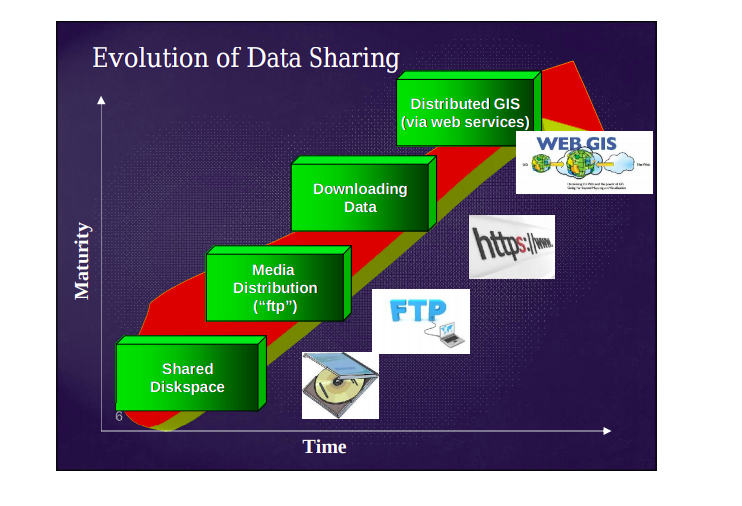
\includegraphics[width=1\textwidth]{images/evolution_projetGIS.png}
        \caption{Cheminement de la solution}
    \end{figure}

\section{Perspective de réalisation}